\section{On-policy distillation}
\label{sec:on-policy-distillation}

On-policy distillation (OPD) asks a fixed teacher to evaluate states reached by a student,
rather than asking the student to imitate completed teacher trajectories. This summary
follows Thinking Machines Lab's formulation \citep{lu2025onpolicydistillation}.

\subsection{Student states with dense teacher feedback}

Offline distillation is dense but trains only on teacher-generated prefixes, so an early
student error can enter an unseen state. Outcome-reward RL samples student states, but its
terminal score does not localize the mistake. OPD retains the student trajectory and asks
the teacher to score every sampled token under its exact student-generated prefix.

The teacher does not replace the rollout. It asks how plausible the next token was given
the student's exact prefix. Figure~\ref{fig:opd-token-feedback} shows an early redirecting
token receiving a strong penalty while the now-predictable final error receives little.

\begin{figure}[htbp]
  \centering
  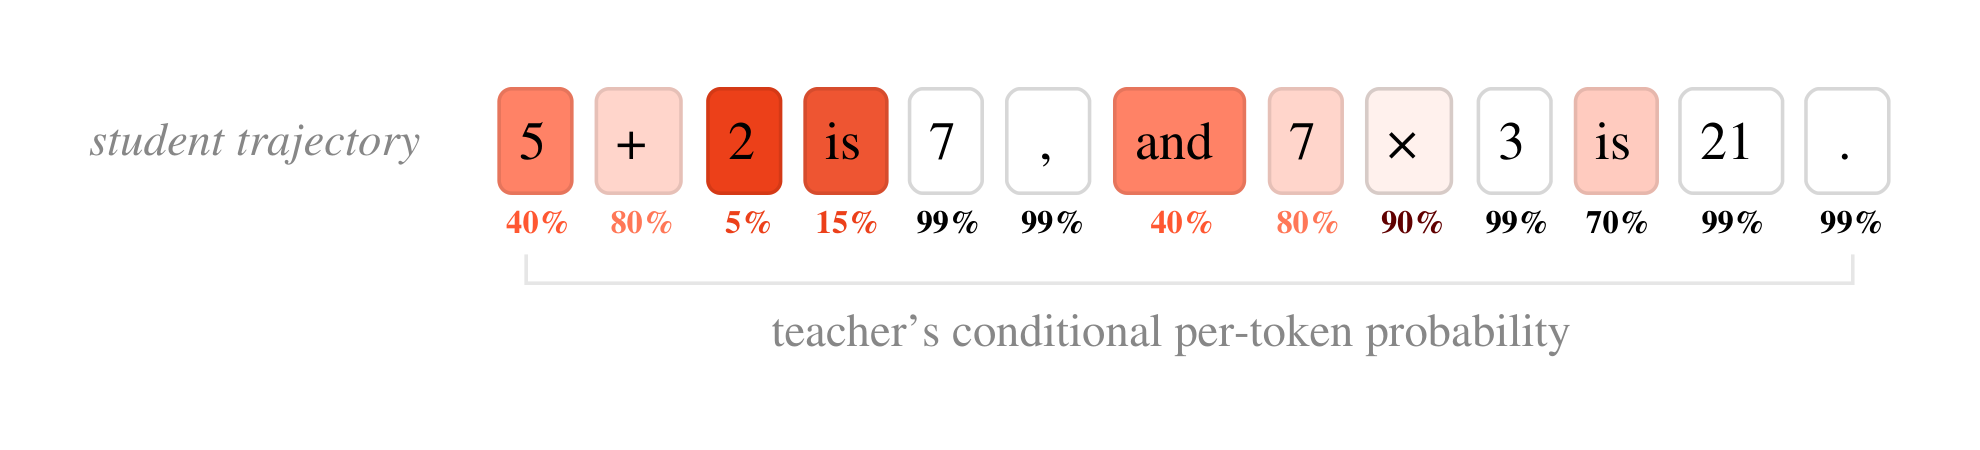
\includegraphics[width=0.88\textwidth]{figures/thinking_machines_opd_token_feedback.png}
  \caption{Teacher probabilities for each token in a student trajectory; darker red means
  lower probability under the exact student prefix. Reproduced from Thinking Machines
  Lab \citep{lu2025onpolicydistillation}.}
  \label{fig:opd-token-feedback}
\end{figure}

\subsection{Reverse-KL training algorithm}

At prefix $s_t$, OPD asks the student's next-token distribution to approach the teacher's
distribution at the same prefix. Thinking Machines Lab uses reverse KL:
\begin{equation}
  D_{\mathrm{KL}}\!\left(\pi_\theta(\cdot\mid s_t)
  \,\|\,\pi_T(\cdot\mid s_t)\right)
  =\mathbb{E}_{a\sim\pi_\theta}
  \left[\log\pi_\theta(a\mid s_t)-\log\pi_T(a\mid s_t)\right].
  \label{eq:opd-reverse-kl}
\end{equation}
The value is zero when the next-token distributions match. Reverse KL is mode-seeking: it
concentrates the student on behavior the teacher considers likely.

The implementation does not need to sample a new answer from the teacher. It performs four
steps:
\begin{enumerate}
  \item Sample exact token trajectories from a student snapshot $\pi_{\mathrm{old}}$ and
        retain the sampled tokens' log-probabilities.
  \item Run the teacher on the same prefixes and record its log-probability for each
        student-sampled token.
  \item Set $A_t=\log\pi_T(a_t\mid s_t)-\log\pi_{\mathrm{old}}(a_t\mid s_t)$: teacher-like
        tokens receive positive signal and implausible tokens receive negative signal.
  \item Update only the student. For reused rollouts, weight $A_t$ by the RL importance
        ratio $\pi_\theta(a_t\mid s_t)/\pi_{\mathrm{old}}(a_t\mid s_t)$.
\end{enumerate}
Prompt, padding, and tool-response tokens remain conditioning context but are masked from
the policy loss. Unlike a terminal advantage broadcast over a whole answer, $A_t$ changes
at every trained token.

\subsection{Initialization, efficiency, and limits}

OPD is most useful when the student already has the relevant capability in its sampling
support and a trustworthy teacher is available. A teacher forward pass supplies feedback
at every token, partial rollouts can be trained without waiting for a terminal verifier,
and no separate reward model is required. In the reported reasoning experiment, OPD raised
AIME'24 accuracy from roughly $60\%$ to $70\%$ using about 77,000 prompts after the SFT
initialization; the article's compute comparisons favor OPD, but depend on its models,
systems, and accounting assumptions \citep{lu2025onpolicydistillation}.

Dense feedback does not create missing support. If the student almost never samples the
teacher's useful strategy, the teacher receives no visited state on which to reinforce it;
SFT or mid-training may first be needed to introduce that behavior. OPD also inherits the
teacher's errors and can reduce useful diversity through reverse-KL mode seeking. It is
therefore better viewed as efficient behavior transfer or recovery on student-visited
states, while RL remains necessary when success must be discovered or judged by an
external environment rather than copied from a teacher.

